\documentclass[]{article}
\usepackage{lmodern}
\usepackage{amssymb,amsmath}
\usepackage{ifxetex,ifluatex}
\usepackage{fixltx2e} % provides \textsubscript
\ifnum 0\ifxetex 1\fi\ifluatex 1\fi=0 % if pdftex
  \usepackage[T1]{fontenc}
  \usepackage[utf8]{inputenc}
\else % if luatex or xelatex
  \ifxetex
    \usepackage{mathspec}
  \else
    \usepackage{fontspec}
  \fi
  \defaultfontfeatures{Ligatures=TeX,Scale=MatchLowercase}
\fi
% use upquote if available, for straight quotes in verbatim environments
\IfFileExists{upquote.sty}{\usepackage{upquote}}{}
% use microtype if available
\IfFileExists{microtype.sty}{%
\usepackage{microtype}
\UseMicrotypeSet[protrusion]{basicmath} % disable protrusion for tt fonts
}{}
\usepackage[margin=1in]{geometry}
\usepackage{hyperref}
\hypersetup{unicode=true,
            pdftitle={Clustering Exercise - HK District Data},
            pdfborder={0 0 0},
            breaklinks=true}
\urlstyle{same}  % don't use monospace font for urls
\usepackage{color}
\usepackage{fancyvrb}
\newcommand{\VerbBar}{|}
\newcommand{\VERB}{\Verb[commandchars=\\\{\}]}
\DefineVerbatimEnvironment{Highlighting}{Verbatim}{commandchars=\\\{\}}
% Add ',fontsize=\small' for more characters per line
\usepackage{framed}
\definecolor{shadecolor}{RGB}{248,248,248}
\newenvironment{Shaded}{\begin{snugshade}}{\end{snugshade}}
\newcommand{\AlertTok}[1]{\textcolor[rgb]{0.94,0.16,0.16}{#1}}
\newcommand{\AnnotationTok}[1]{\textcolor[rgb]{0.56,0.35,0.01}{\textbf{\textit{#1}}}}
\newcommand{\AttributeTok}[1]{\textcolor[rgb]{0.77,0.63,0.00}{#1}}
\newcommand{\BaseNTok}[1]{\textcolor[rgb]{0.00,0.00,0.81}{#1}}
\newcommand{\BuiltInTok}[1]{#1}
\newcommand{\CharTok}[1]{\textcolor[rgb]{0.31,0.60,0.02}{#1}}
\newcommand{\CommentTok}[1]{\textcolor[rgb]{0.56,0.35,0.01}{\textit{#1}}}
\newcommand{\CommentVarTok}[1]{\textcolor[rgb]{0.56,0.35,0.01}{\textbf{\textit{#1}}}}
\newcommand{\ConstantTok}[1]{\textcolor[rgb]{0.00,0.00,0.00}{#1}}
\newcommand{\ControlFlowTok}[1]{\textcolor[rgb]{0.13,0.29,0.53}{\textbf{#1}}}
\newcommand{\DataTypeTok}[1]{\textcolor[rgb]{0.13,0.29,0.53}{#1}}
\newcommand{\DecValTok}[1]{\textcolor[rgb]{0.00,0.00,0.81}{#1}}
\newcommand{\DocumentationTok}[1]{\textcolor[rgb]{0.56,0.35,0.01}{\textbf{\textit{#1}}}}
\newcommand{\ErrorTok}[1]{\textcolor[rgb]{0.64,0.00,0.00}{\textbf{#1}}}
\newcommand{\ExtensionTok}[1]{#1}
\newcommand{\FloatTok}[1]{\textcolor[rgb]{0.00,0.00,0.81}{#1}}
\newcommand{\FunctionTok}[1]{\textcolor[rgb]{0.00,0.00,0.00}{#1}}
\newcommand{\ImportTok}[1]{#1}
\newcommand{\InformationTok}[1]{\textcolor[rgb]{0.56,0.35,0.01}{\textbf{\textit{#1}}}}
\newcommand{\KeywordTok}[1]{\textcolor[rgb]{0.13,0.29,0.53}{\textbf{#1}}}
\newcommand{\NormalTok}[1]{#1}
\newcommand{\OperatorTok}[1]{\textcolor[rgb]{0.81,0.36,0.00}{\textbf{#1}}}
\newcommand{\OtherTok}[1]{\textcolor[rgb]{0.56,0.35,0.01}{#1}}
\newcommand{\PreprocessorTok}[1]{\textcolor[rgb]{0.56,0.35,0.01}{\textit{#1}}}
\newcommand{\RegionMarkerTok}[1]{#1}
\newcommand{\SpecialCharTok}[1]{\textcolor[rgb]{0.00,0.00,0.00}{#1}}
\newcommand{\SpecialStringTok}[1]{\textcolor[rgb]{0.31,0.60,0.02}{#1}}
\newcommand{\StringTok}[1]{\textcolor[rgb]{0.31,0.60,0.02}{#1}}
\newcommand{\VariableTok}[1]{\textcolor[rgb]{0.00,0.00,0.00}{#1}}
\newcommand{\VerbatimStringTok}[1]{\textcolor[rgb]{0.31,0.60,0.02}{#1}}
\newcommand{\WarningTok}[1]{\textcolor[rgb]{0.56,0.35,0.01}{\textbf{\textit{#1}}}}
\usepackage{graphicx,grffile}
\makeatletter
\def\maxwidth{\ifdim\Gin@nat@width>\linewidth\linewidth\else\Gin@nat@width\fi}
\def\maxheight{\ifdim\Gin@nat@height>\textheight\textheight\else\Gin@nat@height\fi}
\makeatother
% Scale images if necessary, so that they will not overflow the page
% margins by default, and it is still possible to overwrite the defaults
% using explicit options in \includegraphics[width, height, ...]{}
\setkeys{Gin}{width=\maxwidth,height=\maxheight,keepaspectratio}
\IfFileExists{parskip.sty}{%
\usepackage{parskip}
}{% else
\setlength{\parindent}{0pt}
\setlength{\parskip}{6pt plus 2pt minus 1pt}
}
\setlength{\emergencystretch}{3em}  % prevent overfull lines
\providecommand{\tightlist}{%
  \setlength{\itemsep}{0pt}\setlength{\parskip}{0pt}}
\setcounter{secnumdepth}{0}
% Redefines (sub)paragraphs to behave more like sections
\ifx\paragraph\undefined\else
\let\oldparagraph\paragraph
\renewcommand{\paragraph}[1]{\oldparagraph{#1}\mbox{}}
\fi
\ifx\subparagraph\undefined\else
\let\oldsubparagraph\subparagraph
\renewcommand{\subparagraph}[1]{\oldsubparagraph{#1}\mbox{}}
\fi

%%% Use protect on footnotes to avoid problems with footnotes in titles
\let\rmarkdownfootnote\footnote%
\def\footnote{\protect\rmarkdownfootnote}

%%% Change title format to be more compact
\usepackage{titling}

% Create subtitle command for use in maketitle
\providecommand{\subtitle}[1]{
  \posttitle{
    \begin{center}\large#1\end{center}
    }
}

\setlength{\droptitle}{-2em}

  \title{Clustering Exercise - HK District Data}
    \pretitle{\vspace{\droptitle}\centering\huge}
  \posttitle{\par}
    \author{}
    \preauthor{}\postauthor{}
    \date{}
    \predate{}\postdate{}
  

\begin{document}
\maketitle

\begin{Shaded}
\begin{Highlighting}[]
\CommentTok{# Load packages}
\KeywordTok{library}\NormalTok{(tidyverse)}
\end{Highlighting}
\end{Shaded}

\begin{verbatim}
## Registered S3 methods overwritten by 'ggplot2':
##   method         from 
##   [.quosures     rlang
##   c.quosures     rlang
##   print.quosures rlang
\end{verbatim}

\begin{verbatim}
## -- Attaching packages --------------------------------------- tidyverse 1.2.1 --
\end{verbatim}

\begin{verbatim}
## v ggplot2 3.1.1     v purrr   0.3.2
## v tibble  2.1.1     v dplyr   0.8.1
## v tidyr   0.8.3     v stringr 1.4.0
## v readr   1.3.1     v forcats 0.4.0
\end{verbatim}

\begin{verbatim}
## -- Conflicts ------------------------------------------ tidyverse_conflicts() --
## x dplyr::filter() masks stats::filter()
## x dplyr::lag()    masks stats::lag()
\end{verbatim}

The dataset for this exercise is from
\href{https://www.bycensus2016.gov.hk/en/}{Hong Kong 2016 Census}. It
lists the average income and median age under different district
councils in Hong Kong.

\hypertarget{prepare-and-explore-data}{%
\subsection{1. Prepare and Explore
Data}\label{prepare-and-explore-data}}

\begin{Shaded}
\begin{Highlighting}[]
\CommentTok{# 2. Load data file}
\NormalTok{df <-}\StringTok{ }\KeywordTok{read_csv}\NormalTok{(}\StringTok{"district_data.csv"}\NormalTok{)}
\end{Highlighting}
\end{Shaded}

\begin{verbatim}
## Parsed with column specification:
## cols(
##   district = col_character(),
##   income = col_character(),
##   age = col_double()
## )
\end{verbatim}

\begin{Shaded}
\begin{Highlighting}[]
\CommentTok{# check first a few rows}
\KeywordTok{head}\NormalTok{(df)}
\end{Highlighting}
\end{Shaded}

\begin{verbatim}
## # A tibble: 6 x 3
##   district            income    age
##   <chr>               <chr>   <dbl>
## 1 Central and Western $17,000  43.8
## 2 Wan Chai            $15,000  44.9
## 3 Eastern             $15,000  43.8
## 4 Southern            $14,500  43.9
## 5 Yau Tsim Mong       $14,500  43.2
## 6 Sham Shui Po        $13,500  42.9
\end{verbatim}

\begin{Shaded}
\begin{Highlighting}[]
\CommentTok{# check the dimension of data}
\KeywordTok{dim}\NormalTok{(df)}
\end{Highlighting}
\end{Shaded}

\begin{verbatim}
## [1] 18  3
\end{verbatim}

\begin{Shaded}
\begin{Highlighting}[]
\CommentTok{# check the summary of data}
\KeywordTok{summary}\NormalTok{(df)}
\end{Highlighting}
\end{Shaded}

\begin{verbatim}
##    district            income               age       
##  Length:18          Length:18          Min.   :42.10  
##  Class :character   Class :character   1st Qu.:42.95  
##  Mode  :character   Mode  :character   Median :43.55  
##                                        Mean   :43.46  
##                                        3rd Qu.:43.80  
##                                        Max.   :44.90
\end{verbatim}

\hypertarget{data-cleaning}{%
\subsection{2. Data Cleaning}\label{data-cleaning}}

\begin{Shaded}
\begin{Highlighting}[]
\CommentTok{# check column names}
\KeywordTok{names}\NormalTok{(df)}
\end{Highlighting}
\end{Shaded}

\begin{verbatim}
## [1] "district" "income"   "age"
\end{verbatim}

\begin{Shaded}
\begin{Highlighting}[]
\CommentTok{# rename the column names}
\KeywordTok{names}\NormalTok{(df) <-}\StringTok{ }\KeywordTok{c}\NormalTok{(}\StringTok{"district"}\NormalTok{, }\StringTok{"avg_income"}\NormalTok{, }\StringTok{"median_age"}\NormalTok{)}
\KeywordTok{names}\NormalTok{(df)}
\end{Highlighting}
\end{Shaded}

\begin{verbatim}
## [1] "district"   "avg_income" "median_age"
\end{verbatim}

The data type of \texttt{avg\_income} column is string now, so we need
to convert it to numeric.

\begin{Shaded}
\begin{Highlighting}[]
\CommentTok{# remove $ and thousand separator}
\NormalTok{df}\OperatorTok{$}\NormalTok{avg_income <-}\StringTok{ }\KeywordTok{gsub}\NormalTok{(}\StringTok{"[$,]"}\NormalTok{, }\StringTok{""}\NormalTok{, df}\OperatorTok{$}\NormalTok{avg_income)}

\CommentTok{# convert to numeric}
\NormalTok{df}\OperatorTok{$}\NormalTok{avg_income <-}\StringTok{ }\KeywordTok{as.numeric}\NormalTok{(df}\OperatorTok{$}\NormalTok{avg_income)}

\CommentTok{# check the column types}
\KeywordTok{glimpse}\NormalTok{(df)}
\end{Highlighting}
\end{Shaded}

\begin{verbatim}
## Observations: 18
## Variables: 3
## $ district   <chr> "Central and Western", "Wan Chai", "Eastern", "Sout...
## $ avg_income <dbl> 17000, 15000, 15000, 14500, 14500, 13500, 15000, 14...
## $ median_age <dbl> 43.8, 44.9, 43.8, 43.9, 43.2, 42.9, 43.1, 44.6, 43....
\end{verbatim}

\hypertarget{data-visualization}{%
\subsection{3. Data Visualization}\label{data-visualization}}

\begin{Shaded}
\begin{Highlighting}[]
\KeywordTok{qplot}\NormalTok{(}\DataTypeTok{x =}\NormalTok{ df}\OperatorTok{$}\NormalTok{median_age, }\DataTypeTok{y =}\NormalTok{ df}\OperatorTok{$}\NormalTok{avg_income, }\DataTypeTok{label =}\NormalTok{ df}\OperatorTok{$}\NormalTok{district, }\DataTypeTok{geom =} \StringTok{"text"}\NormalTok{)}
\end{Highlighting}
\end{Shaded}

\includegraphics{exercise_hk_district_files/figure-latex/unnamed-chunk-7-1.pdf}

\hypertarget{k-means-clustering}{%
\subsection{4. K-means Clustering}\label{k-means-clustering}}

Because the income data is in thousand, much `bigger' than age data, so
we need to scale the income data before clustering.

\begin{Shaded}
\begin{Highlighting}[]
\NormalTok{df_scaled <-}\StringTok{ }\KeywordTok{as.data.frame}\NormalTok{(}\KeywordTok{scale}\NormalTok{(df[}\KeywordTok{c}\NormalTok{(}\StringTok{"median_age"}\NormalTok{, }\StringTok{"avg_income"}\NormalTok{)]))}

\KeywordTok{head}\NormalTok{(df_scaled)}
\end{Highlighting}
\end{Shaded}

\begin{verbatim}
##   median_age avg_income
## 1  0.4706704  2.4607693
## 2  1.9737792  0.2020315
## 3  0.4706704  0.2020315
## 4  0.6073167 -0.3626529
## 5 -0.3492071 -0.3626529
## 6 -0.7591459 -1.4920218
\end{verbatim}

\begin{Shaded}
\begin{Highlighting}[]
\CommentTok{# define the number of clusters}
\NormalTok{k_clusters <-}\StringTok{ }\DecValTok{3}

\CommentTok{# get clustering result}
\NormalTok{k_means_result <-}\StringTok{ }\KeywordTok{kmeans}\NormalTok{(df_scaled, }\DataTypeTok{centers =}\NormalTok{ k_clusters)}

\CommentTok{# add cluster result to original data}
\NormalTok{df}\OperatorTok{$}\NormalTok{cluster <-}\StringTok{ }\KeywordTok{as.factor}\NormalTok{(k_means_result}\OperatorTok{$}\NormalTok{cluster)}

\KeywordTok{head}\NormalTok{(df)}
\end{Highlighting}
\end{Shaded}

\begin{verbatim}
## # A tibble: 6 x 4
##   district            avg_income median_age cluster
##   <chr>                    <dbl>      <dbl> <fct>  
## 1 Central and Western      17000       43.8 3      
## 2 Wan Chai                 15000       44.9 3      
## 3 Eastern                  15000       43.8 2      
## 4 Southern                 14500       43.9 2      
## 5 Yau Tsim Mong            14500       43.2 2      
## 6 Sham Shui Po             13500       42.9 2
\end{verbatim}

\begin{Shaded}
\begin{Highlighting}[]
\CommentTok{# visualize cluster result}
\KeywordTok{qplot}\NormalTok{(}\DataTypeTok{x =}\NormalTok{ df}\OperatorTok{$}\NormalTok{median_age, }\DataTypeTok{y =}\NormalTok{ df}\OperatorTok{$}\NormalTok{avg_income, }\DataTypeTok{label =}\NormalTok{ df}\OperatorTok{$}\NormalTok{district, }\DataTypeTok{geom =} \StringTok{"text"}\NormalTok{, }\DataTypeTok{color =}\NormalTok{ df}\OperatorTok{$}\NormalTok{cluster)}
\end{Highlighting}
\end{Shaded}

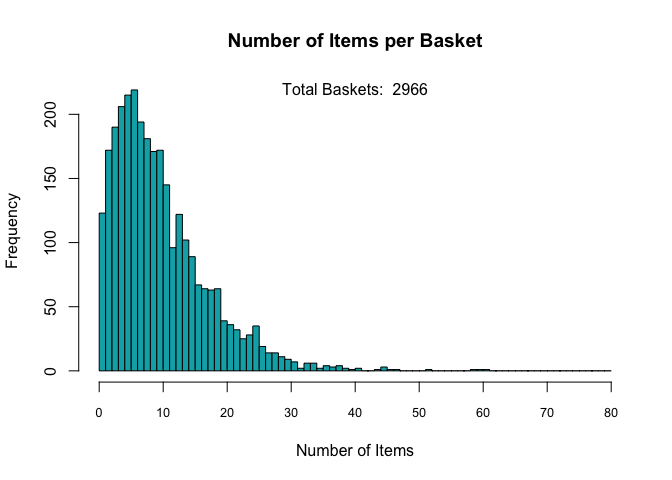
\includegraphics{exercise_hk_district_files/figure-latex/unnamed-chunk-10-1.pdf}

\hypertarget{decide-the-optimal-number-of-clusters}{%
\subsection{5. Decide the optimal number of
clusters}\label{decide-the-optimal-number-of-clusters}}

\begin{Shaded}
\begin{Highlighting}[]
\CommentTok{# set maximum number of cluster}
\NormalTok{k_cluster_max <-}\StringTok{ }\DecValTok{10}
\end{Highlighting}
\end{Shaded}

\begin{Shaded}
\begin{Highlighting}[]
\CommentTok{# iterate through the number of clusters from 1 to 10}
\NormalTok{within_sum_of_squares <-}\StringTok{ }\KeywordTok{sapply}\NormalTok{(}\DecValTok{1}\OperatorTok{:}\NormalTok{k_cluster_max, }
                                \ControlFlowTok{function}\NormalTok{(k)\{}
                                  \KeywordTok{kmeans}\NormalTok{(df_scaled, }\DataTypeTok{centers =}\NormalTok{ k)}\OperatorTok{$}\NormalTok{tot.withinss\})}

\CommentTok{# visualize the output}
\KeywordTok{plot}\NormalTok{(}\DecValTok{1}\OperatorTok{:}\NormalTok{k_cluster_max, within_sum_of_squares, }\DataTypeTok{type =} \StringTok{"b"}\NormalTok{,}
     \DataTypeTok{xlab =} \StringTok{"Number of clusters"}\NormalTok{, }\DataTypeTok{ylab =} \StringTok{"Total within cluster sum of squares"}\NormalTok{)}
\end{Highlighting}
\end{Shaded}

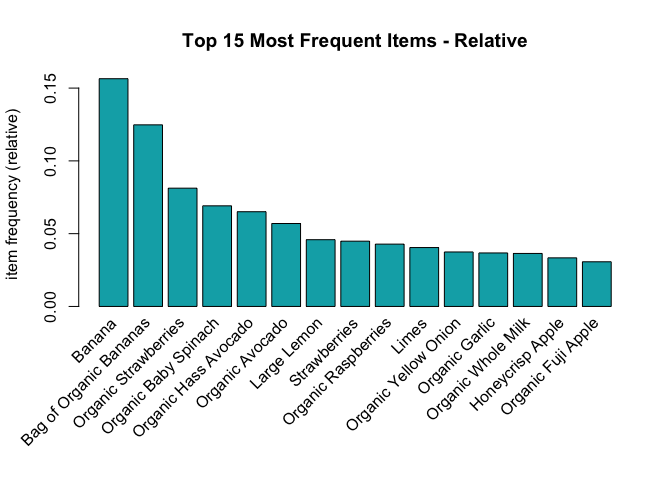
\includegraphics{exercise_hk_district_files/figure-latex/unnamed-chunk-12-1.pdf}

The chart shows that probably 4 is the correct number of clusters as the
curve bents most at this point, so we repeat clustering with 4 clusters.

\begin{Shaded}
\begin{Highlighting}[]
\CommentTok{# conduct clustering with 4 clusters}
\NormalTok{k_means_result_}\DecValTok{2}\NormalTok{ <-}\StringTok{ }\KeywordTok{kmeans}\NormalTok{(df_scaled, }\DataTypeTok{centers =} \DecValTok{4}\NormalTok{)}

\CommentTok{# add result to dataframe}
\NormalTok{df}\OperatorTok{$}\NormalTok{cluster <-}\StringTok{ }\KeywordTok{as.factor}\NormalTok{(k_means_result_}\DecValTok{2}\OperatorTok{$}\NormalTok{cluster)}
\end{Highlighting}
\end{Shaded}

\begin{Shaded}
\begin{Highlighting}[]
\CommentTok{# visualize cluster result with ggrepel to avoid label overlapping}
\KeywordTok{library}\NormalTok{(ggrepel)}
\KeywordTok{qplot}\NormalTok{(}\DataTypeTok{x =}\NormalTok{ df}\OperatorTok{$}\NormalTok{median_age, }\DataTypeTok{y =}\NormalTok{ df}\OperatorTok{$}\NormalTok{avg_income, }\DataTypeTok{label =}\NormalTok{ df}\OperatorTok{$}\NormalTok{district, }\DataTypeTok{color =}\NormalTok{ df}\OperatorTok{$}\NormalTok{cluster,}
      \DataTypeTok{xlab =} \StringTok{"Median Age"}\NormalTok{, }\DataTypeTok{ylab =} \StringTok{"Average Income"}\NormalTok{) }\OperatorTok{+}\StringTok{ }\KeywordTok{geom_text_repel}\NormalTok{()}
\end{Highlighting}
\end{Shaded}

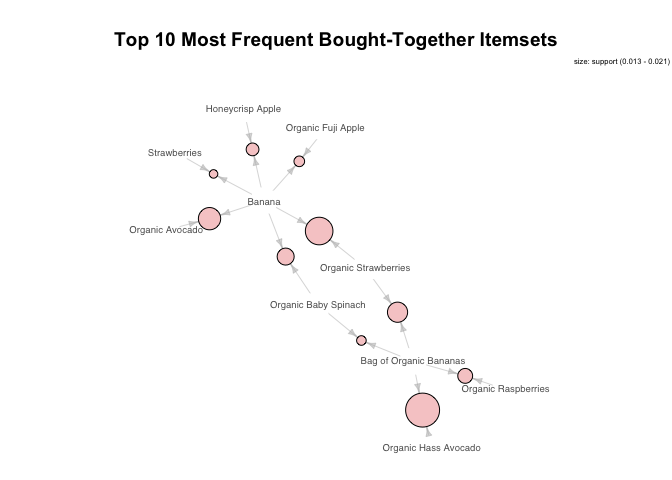
\includegraphics{exercise_hk_district_files/figure-latex/unnamed-chunk-14-1.pdf}

The graph shows that the districts has been allocated to 4 groups, the
result is reasonable and reliable.


\end{document}
